\section{Architecture 101}

%\subsection{}

%\subsubsection{}

\textbf{Architectures:}
\begin{itemize}
	\item The art or practice of \textbf{designing} and \textbf{building} structure and especially habitable ones.
	\item A unifying or coherent \textbf{from} or \textbf{structure}
\end{itemize}

\textbf{Foundation for the study of Software Architecture / L. Wolf, 1992}

Software architecure principles can be \textbf{inherited} by appealing to several well-established architectural disciplines.

While the subject matter for the two is quite different, there are a number of intresting \textbf{architectural points} in building architecture that are suggestive for software architecture
\begin{itemize}
	\item multimple \textbf{views}
	\item architectural \textbf{styles}
	item style and \textbf{materials}
+\end{itemize}

\subsection{Multiple Views}

\subsubsection{Building Architecture}

\textbf{Building Architecture uses MULTIPLE VIEWS}

A building architect works with the customer by means of a number of different views in which sone \textbf{particular aspect of the building} is emphasized.

For exmaple, there are elevations and floor plans that give the \textbf{exterior views} and "\textbf{top-down}" views, respectively.

The elevation views may be supplemented by \textbf{contextual drawings} or even scale models to provide the customer with the look of the building in its context.

\subsubsection{Different Stakeholders}
Each perspective is not just a matter of different level or detail.

It is linked with \textbf{different natures} and \textbf{accountability}.

\begin{itemize}
	\item The \textbf{Owner} needs the building for a specific purpose. He/she does not know how, but hw/she knows perfectly \textbf{why}
	\item The \textbf{Architect} needs to project and formalize something that fit completely with owner's needs, to plan the \textbf{what}
	\item The \textbf{Builder} needs to design \textbf{how} the what will be built matching with natural laws and techological costraints
\end{itemize}

\subsubsection{\sout{Building} Software Architecture}

\textbf{\sout{Building} Software Architecture uses MULTIPLE VIEWS}

Different \textbf{type of users} will use Software Architecture: each of them will need a specific point of view.

A \textbf{Full Stack} developer needs to know how to write code inside the Architecture while a \textbf{Data Scientist} where are data they need.

\begin{center}
	\textit{Since the technology permits \textbf{destributing} large amounts of computing facilities in small packages to \textbf{remote location}, some kind of structure (or architecture) is imperative because \textbf{decentralization without structure is chaos}}.
\end{center}

\subsubsection{Zachman Framework for Building}

\begin{center}
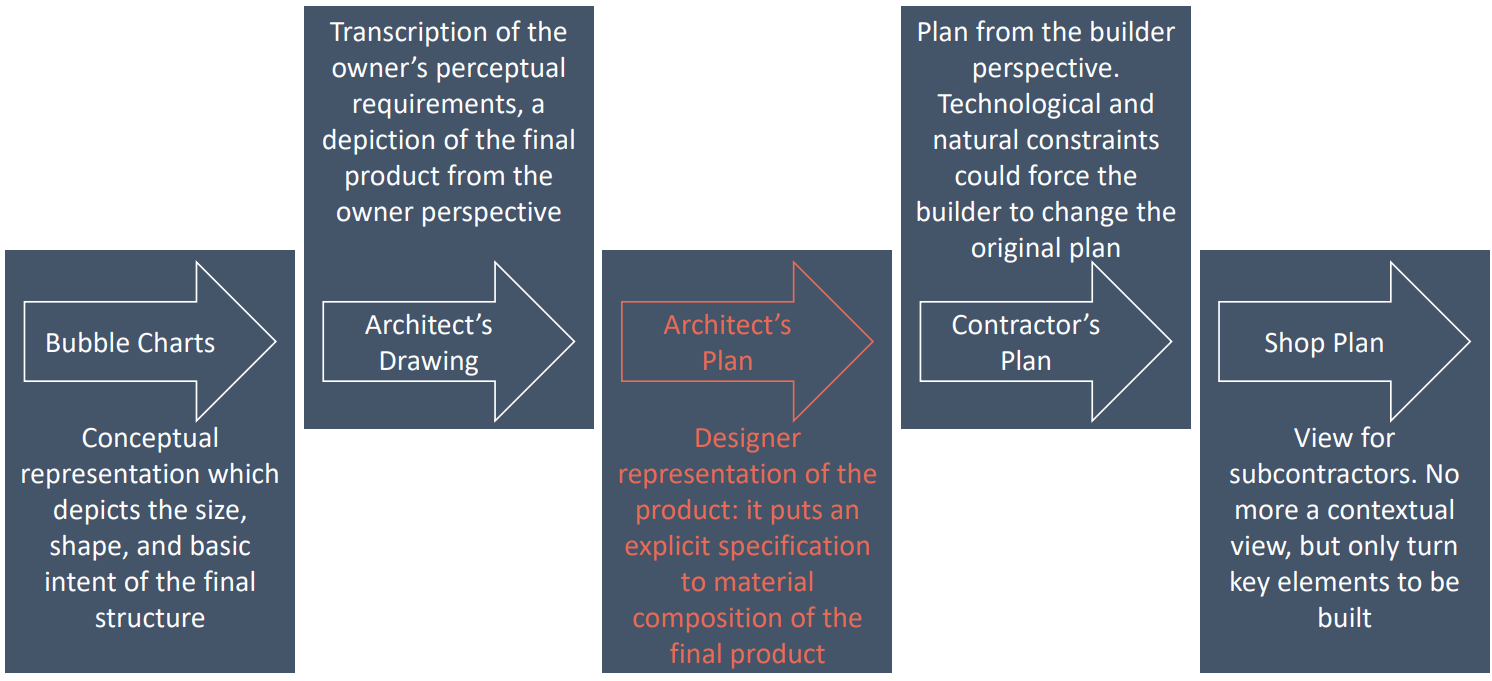
\includegraphics[scale=0.3]{1-zachman-framework-for-building}
\end{center}

\subsubsection{Zachman Framework for Information System}
\begin{center}
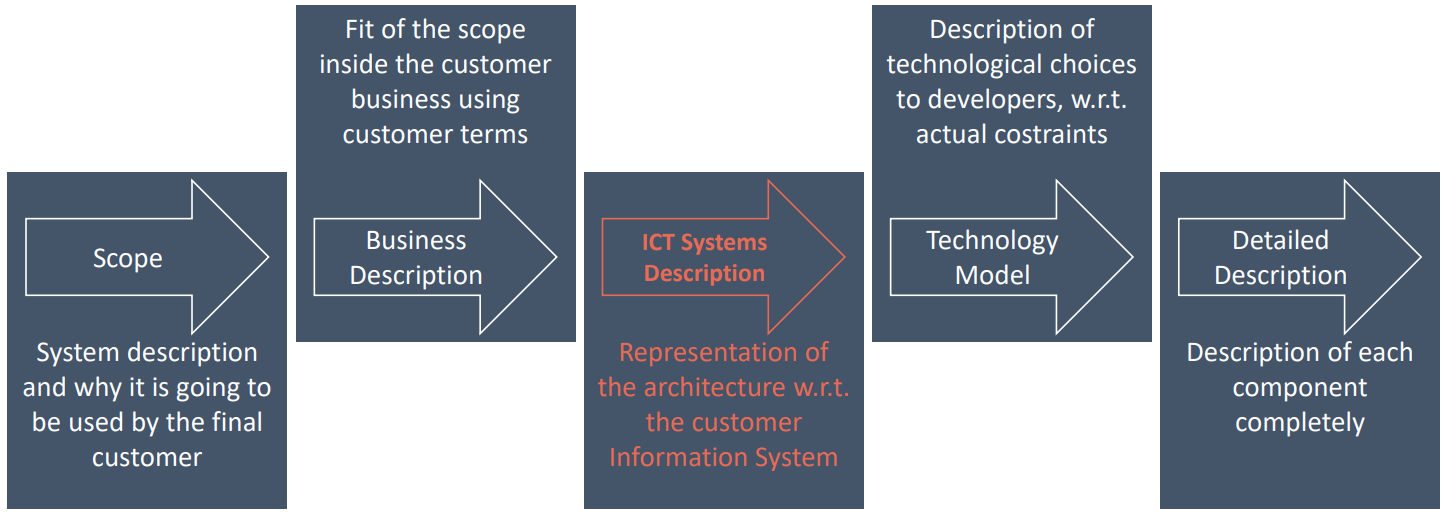
\includegraphics[scale=0.3]{2-zachman-framework-for-information-system}
\end{center}

\subsubsection{Different point of views}
Each perspective is not just a matter of different level of detail.

It is linked with \textbf{different natures} and \textbf{accountability}.

\begin{itemize}
	\item \textbf{Input-Process-Output}
	
	Product description in detail w.r.t. intended capabilities, appearance, and interactions with users
	
	\item \textbf{Entity-Relationship-Entity}
	
	<<Stuff things is made of>>, description of data in each building blocks
	
	\item \textbf{Node-Line-Node}
	
	Flows between each component
\end{itemize}

\subsection{Architectural Styles}

\textbf{Software Architecture}
A software architecture is a set of \textbf{architectural elements} that have a particular form.
\begin{center}
[...]
\end{center}
The architectural form consists of weighted \textbf{properties} and \textbf{relationship}.
\begin{center}
[...]
\end{center}
An underlying, but integral, part of an architecture is the rationale for the various choice made in defining an architecture.

\subsubsection{Building Architecture}
\textbf{Building Architecture exploits different ARCHITECTURAL STYLES}

\textbf{Descriptively}, architectural style defines a particular codification of \textbf{design elements} and formal arrangements.

\textbf{Prescriptively}, style limits the kinds of design elemetns and their \textbf{formal arragements}.

That is, an architectural style constrains both the \textbf{design elements} and the \textbf{formal relationship} among the degign elements.

\subsubsection{\sout{Building} Software Architecture}

\textbf{\sout{Building} Software Architecture exploits different ARCHITECTURAL STYLES}

Architectural Style \textbf{encapsulates} important decision about elements and emphasizes important constraints on them and their relationships. 

We can use Architecture Style both to \textbf{constrain} the architecture and to \textbf{coordinate} cooperating architects.

Moreover, style \textbf{embodies} those decision that suffer \textbf{erosion and drift}: an emphasis on it as a constraint on the architecture provides a visibility to certain aspects of the architecture so that violations of those aspects and insesnsitivity of them will be more obvious.

\subsubsection{Elements}

\begin{center}
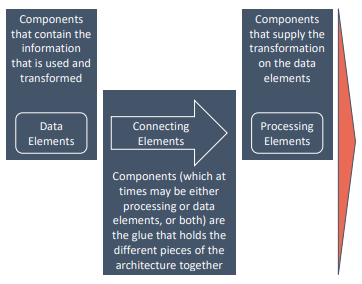
\includegraphics[scale=0.7]{3-architectural-styles-elements}
\end{center}

\textbf{Properties} are used \textbf{to constrain the choice of architectural elements}. They define the minimum desired constraints unless otherwise stated: by default on "what is not constrained by the architect may take any form desired by the designer or implementer"

\textbf{Relationship} are used \textbf{to constrain the "placement" of architectural element} - how the different elements may interact and how they are organized with respect to each other in the architecture

\textbf{Rationale} is an underlying. but integral, part of an architecture for the various choices mad in defining an acrchitexture. \textbf{It captures the motivation for the choice of architectural style, the choice of elements, and the form to satisfy the system constraints}

\subsubsection{Enterprise Architecture Styles}

\begin{enumerate}
	\item \textbf{\textit{1990 - Common Object Request Broker Architecture - COBRA}}
	\textit{"Framework to allow objects hosted in different systems to make remote procedures call via a computer network using an Object Request Broker which marshals and serializes these requests"}	
	
	\item \textbf{\textit{2003 - Service Oriented Architecture - SOA}}
	\textit{"Framework for integrating business processes and supporting IT infrastructure as secure, standardized components - services - that can be reused and combined to address changing business priorities"} Bieberstein, Bose et al. 2005
	
	1. 2012 - Microservices
	
	\item \textbf{\textit{2004 - Message Oriented Architecture - MOM}}
	"Framework to allow objects hosted in different systems to send messages via a computer network using Message Broker to distribuite Application modules over heterogeneous platform"

	\item ...	
\end{enumerate}

\subsection{Style and Material}

\subsubsection{Building Architecture}

\textbf{Classical Architecture combines STYLE and MATERIALS}

The materials have \textbf{certain properties} that are exploited in providing a particular style. One may combine structural with aesthetic uses of materials, such as that found in the post and beam construction of tudor-style houses.

However, \textbf{one does not build a skyscraper with wooden posts} and beams.

The \textbf{material aspects} of the design elements provide both aesthetic and engineering bases for an architecture.

\subsubsection{\sout{Building} Software Architecture}

\textbf{\sout{Building} Software Architecture combines STYLE and MATERIALS}

The same function can be obtained using \textbf{different subsystems}.

To train a \textbf{Neural Network Python} could be the best fit, while to put the trained Network in production using \textbf{FPGA} to physically build the network could be a better solution.

\subsection{When an Architecture is designed}
\begin{center}
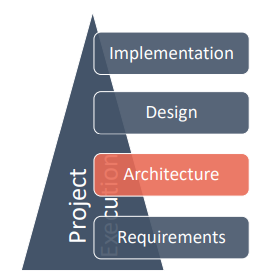
\includegraphics[scale=0.7]{4-when-an-architecture-is-designed}
\end{center}

\begin{itemize}
	\item Implementation: Representations of the algorithms and data types that satisfy the \textbf{design, architecture} and \textbf{requirements}
	
	\item Design: Modularization and detailed interfaces of the design elements, their algorithms and procedures, and the data types needed to support the \textbf{architecture} and to satisfy the requirements.
	
	\item Architecture: Selection of \textbf{architectural elements}, thier \textbf{interactions}, and the \textbf{constraints} to provide a framework in which to satisfy the \textbf{requirements} and serve as a basis for the \textbf{design}
	
	\item Requirements: Determination of the information, processing, and the characteristics of that information and processing needed by the user of the system
\end{itemize}

There new problems involve the system-level design of software, in which the important decisions are concerned with the kinds of modules and subsystems to use and the may these modules and subsystems are organized.

This level of organization, the software architecutre level, requires new kinds of abstractions that capture essential properties of major subsystems and the ways thay interact.

\subsection{Architecture as a framework for abstractions}
\begin{itemize}
	\item The essence of \textbf{abstraction} is recognizing a pattern, naming and defining it, analyzing it, inding ways to specify it, and providing some way to invoke the pattern by its name without error-prone manual intervention
	\item This process \textbf{suppresses the detail of the pattern's implementation}, reduces the opportunity for clerical error, and simplifies understanding of the result
	\item In other words, good abstraction is \textbf{ignoring the right detail} at the right times
\end{itemize}

\textit{"The development of \textbf{individual abstractions} often follows a common pattern:}
\begin{itemize}
	\item \textit{First, problems are \textbf{solved ad hoc}}
	\item \textit{As experience accumulates, some solutions turn out to work better than others, and \textbf{a sort of solklore is passed informally} from person to person}
	\item \textit{Eventually the useful solutions are understood more systematically, and they are \textbf{codified} and analyzed}
	\item \textit{This in turn enables \textbf{a more sphisticated level of} practice and allows us to tackle harder problems"}
\end{itemize}

\subsubsection{Example of Abstraction}

\begin{center}

\textbf{First example}

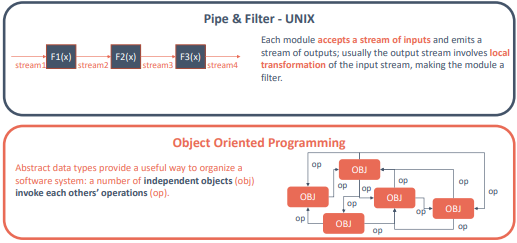
\includegraphics[scale=0.7]{5-example-of-abstraction}

\textbf{Second example}

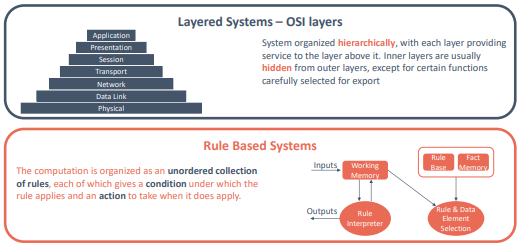
\includegraphics[scale=0.7]{6-example-of-abstraction}
\end{center}

\subsubsection{System-subsystem Abstraction}

System are constructed by combining \textbf{subsystems}:
\begin{itemize}
	\item indipendently \textbf{compilable modules}, linked by shared data or procedure calls
	\item sets of \textbf{design decisions} and the \textbf{code} that implements them
	
Subsystem \textbf{have an internal structure}. It is often useful to design that substructure at an architectural level before implementing it
\end{itemize}

Each subsystem may performs:
\begin{itemize}
	\item a \textbf{specific function} to the system begin implemented
	\item a \textbf{more common function} such as communication or storage
\end{itemize}

\textbf{Identifying} and \textbf{classifying} the system functions that are common to many applications is a significant first step to the development of a software architecture.